\documentclass[matan.tex]{subfiles}

\begin{document}
     \begin{lect} {11.10.19}
        \section{Условные экстремумы}
        \[u = f(x_1, ..., x_n) \text{ при усл } \begin{cases}
            \Phi_1 (x_1, ..., x_n) = 0\\
            \vdots\\
            \Phi_m (x_1, ..., x_n) = 0
        \end{cases} \q m < n\]
        \begin{enumerate}
            \item Точка недифф-ти $f$ или $\Phi_i$
            \item $\rk \Phi' < m$
                \[\Phi' = \begin{pmatrix}
            \frac{\partial \Phi_1}{\partial x_1} & ... & \frac{\partial \Phi_1}{\partial x_n}\\
            \vdots & & \vdots\\
            \frac{\partial \Phi_m}{\partial x_1} & ... & \frac{\partial \Phi_m}{\partial x_n}
        \end{pmatrix} \qq m \times n\]
            \item $\LL = f(x_1, ..., x_n) - \lambda_1 \Phi_1 (x_1, ..., x_n) - 
                \lambda_2 \Phi_2 (x_1, ..., x_n) - ... -\lambda_m \Phi_m(x_1, ..., x_n)$
        \end{enumerate}
            
        
        Точка экстремума удовлетворяет системе уравнений:
        \[\begin{cases}
                \frac{\partial \LL}{\partial x_1} = 0\\
                \vdots\\
                \frac{\partial \LL}{\partial x_n} = 0\\
                \Phi_1(x_1, ..., x_n) = 0\\
                \vdots\\
                \Phi_m(x_1, ..., x_n) = 0
        \end{cases} \qq m + n \text{ уравнений } \q \]
        \[m + n \text{ неизвестных} \q x_1, ..., x_n, \lambda_1, ..., \lambda_m\]

        \begin{Task}[1]
            \[f(x, y) = \frac{x}{a} + \frac{y}{b} \qq a, b > 0 \text{ при усл. } x^2 + y^2 = 1 \rla \underbracket{x^2 + y^2 - 1}_{\Phi} = 0 \qq M \]
            \[\Phi' = \begin{pmatrix}
                2x & 2y
            \end{pmatrix} \qq \text{1 ур-е } \Ra \text{1 строка в матрице}\]
            \[\rk \Phi' < 1 \Ra \rk \Phi'  = 0  \q\Ra \begin{cases}
                    x = 0\\
                    y = 0
            \end{cases} \cancel{\in } M\]
            \[\forall (x, y) \in M \qq \rk \Phi' = 1\]
            \[\LL = \frac{x}{a} + \frac{y}{b} - \lambda(x^2 + y^2 - 1)\]
            \[\begin{cases}
                \LL'_x = \frac{1}{a} - 2\lambda \cdot x = 0 \Ra \lambda \neq 0 \qq &x = \frac{1}{2a\lambda}\\
                \LL'_y = \frac{1}{b} - 2\lambda \cdot y = 0 \Ra &y = \frac{1}{2b\lambda}\\
                x^2 + y^2 = 1       
            \end{cases}\] 
            \[\frac{1}{4a^2\lambda^2} + \frac{1}{4b^2\lambda^2} = 1\]
            \[\frac{b^2 + a^2}{4a^2b^2\lambda^2} = 1\]
            \[a^2 + b^2 = 4a^2b^2 \lambda^2\]
            \[\lambda = \pm \frac{\sqrt{a^2 + b^2}}{2ab}\]
            \[1.\begin{cases}
                x = \frac{1 \cdot 2 ab}{2a \sqrt{a^2 + b^2}} = \frac{b}{\sqrt{a^2 + b^2}}\\
                y = \frac{a}{\sqrt{a^2 + b^2}}\\
                \lambda = +\frac{\sqrt{a^2 + b^2}}{2ab}
            \end{cases}\]
            \[2.\begin{cases}
                x = -\frac{b}{\sqrt{a^2 + b^2}}\\
                y = - \frac{a}{\sqrt{ a^2 + b^2}}\\
                \lambda = -\frac{\sqrt{a^2 + b^2}}{2ab}
            \end{cases}\]  
            Выясним, что будет в этих точках
            \[\LL_{x^2}'' = -2\lambda\]
            \[\LL_{xy}'' = 0 \]
            \[\LL_{y^2}'' = -2\lambda\]
            \[\begin{pmatrix}
                -2\lambda & 0\\
                0   & -2 \lambda
            \end{pmatrix} \qq \Delta_1 = 2\lambda \q \Delta_2 = 4\lambda^2\]
            \[\begin{matrix}
                \text{для } & 1. & - & + & \max\\
                            & 2. & + & + & \min
            \end{matrix}\]
        \end{Task}

        \begin{Task}[2]
            \[u = x^2 + y^2 + z^2\]
            \[\frac{x^2}{a^2} + \frac{y^2}{b^2} + \frac{z^2}{c^2} = 1 \qq a > b > c > 0\]
            \[\frac{x^2}{a^2} + \frac{y^2}{b^2} + \frac{z^2}{c^2} - 1 = 0\]
            \[\Phi' = \begin{pmatrix}
                \frac{2x}{a^2} & \frac{2y}{b^2} & \frac{2z}{c^2}
            \end{pmatrix}\]
            \[\rk \Phi' = 0  \Ra \q x = y = z = 0 \qq (0, 0, 0) \cancel{\in } M\]
            \[\LL = x^2 + y^2 + z^2 - \lambda(\frac{x^2}{a^2} + \frac{y^2}{b^2} + 
            \frac{z^2}{c^2} - 1)\]
            \[\begin{cases}
                \LL_x' = 2x - \frac{2x\lambda}{a^2} = 0 
                \Ra x(1 - \frac{\lambda}{a^2}) = 0\\
                \LL'_y = 2y - \frac{2y\lambda}{b^2} = 0 
                \Ra y(1 - \frac{\lambda}{b^2}) = 0\\
                \LL'_z = 2z - \frac{2z\lambda}{c^2} = 0
                \Ra z(1 - \frac{\lambda}{c^2}) = 0\\
                \frac{x^2}{a^2} + \frac{y^2}{b^2} + \frac{z^2}{c^2} = 1
            \end{cases}\]
            \[1 - \frac{\lambda}{b^2} = 0 \Ra \lambda = b^2\]
            \[x = z = 0 \qq y \pm b\]
            \[1 - \frac{\lambda}{c^2} = 0 \Ra \lambda = c^2\]
            \[x = y = 0 \qq z = \pm c\]
            \[1 - \frac{\lambda}{a^2} = 0\]
            \[\lambda = a^2  \qq 1 - \frac{a^2}{b^2} \neq 0\]
            \[\Ra y = 0\]
            \[1 - \frac{a^2}{c^2} \neq 0 \Ra z = 0\]
            \[\Ra \frac{x^2}{a^2} = 1\]
            \[\begin{cases}
                x = \pm a\\
                y = 0\\
                z = 0\\
                \lambda = a^2
            \end{cases}\]
            \[\text{6 решений } \begin{matrix}
                \begin{pmatrix}
                    \pm a & 0 & 0 & a^2\\
                \end{pmatrix} \q
                \begin{pmatrix}
                    0 & \pm b & 0 & b^2\\
                \end{pmatrix}\q
                \begin{pmatrix}
                    0 & 0 & \pm c & c^2
                \end{pmatrix}
            \end{matrix}\]
            \[\begin{pmatrix}
                2 - \frac{2\lambda}{a^2} & 0 & 0\\
                0 & 2 - \frac{2\lambda}{b^2} & 0\\
                0 & 0 & 2 - \frac{2\lambda}{c^2}
            \end{pmatrix}\]
            \[\Delta_1 = 2 - \frac{2\lambda}{a^2} = 2(1- \frac{\lambda}{a^2})\]
            \[\Delta_2 = 4(1 - \frac{\lambda}{a^2})(1 - \frac{\lambda}{b^2})\]
            \[\Delta_3 = 8(1 - \frac{\lambda}{a^2})(1 - \frac{\lambda}{b^2})
            (1 - \frac{\lambda}{c^2})\]
            \begin{enumerate}
                \item $\lambda = a^2 \qq 0, \ 0,\  0$
                \item $\lambda = b^2 \qq 1 - \frac{b^2}{a^2} > 0, \ 0, \ 0$
                \item $\lambda = c^2 \qq 1 - \frac{c^2}{a^2} > 0, \ 
                    (1 - \frac{c^2}{a^2})(1 - \frac{c^2}{b^2}) > 0, \ 0$
            \end{enumerate}
            Но у нас $2$ независимые переменные
            \[d^2\LL = 2(1 - \frac{\lambda^2}{a^2})(dx)^2 + 
            2(1 - \frac{\lambda}{b^2})(dy)^2 + 2(1 - \frac{\lambda}{c^2})(dz)^2\]
            \[\frac{2x}{a^2}dx + \frac{2y}{b^2}dy + \frac{2z}{c^2}dz = 0\]
             - линейная однородная система относительно диф-лов
            \[dx, dy, dz \text{ - зависимы между собой}\]
            \[\text{В точке } \begin{pmatrix}
                \pm a, & 0, & 0, & a^2
            \end{pmatrix} \text{ - максимум}\]
            \[\frac{\pm 2a}{a^2}dx = 0 \Ra dx \equiv 0\]
            \[d^2 \LL = 2(1 - \frac{a^2}{b^2})(dy)^2 + 2(1 - \frac{a^2}{c^2})(dz)^2\]
            \[\begin{pmatrix}
                2(1 - \frac{a^2}{b^2}) & 0\\
                0 & 2(1 - \frac{a^2}{c^2})
            \end{pmatrix} \qq \begin{matrix}
                \Delta_1 =& 2(1 - \frac{a^2}{b^2}) < 0\\
                \Delta_2 =& 4 (1 - \frac{a^2}{b^2})(1 - \frac{a^2}{c^2}) > 0\\
                - \q +  &\ul{\text{ максимум }}
            \end{matrix}\]
            \[\text{В точке } \begin{pmatrix}
                0, & \pm b, & 0, & b^2
            \end{pmatrix} \text{ нет экстремума}\]
            \[\pm \frac{2b}{b^2}dy = 0 \Ra dy = 0\]
            \[d^2\LL = 2(1 - \frac{b^2}{a^2})(dx)^2 + 2(1 - \frac{b^2}{c^2})(dz)^2\]
            \[\begin{pmatrix}
                2(1 - \frac{b^2}{a^2}) & 0\\
                0 & 2(1 - \frac{b^2}{c^2})
            \end{pmatrix} \qq \begin{matrix}
                \Delta_1 =& 2(1 - \frac{b^2}{a^2}) > 0\\
                \Delta_2 =& 4(1 - \frac{b^2}{a^2})(1 - \frac{b^2}{c^2}) < 0\\
                + \q - & \ul{\text{ нет экстремума}}
            \end{matrix}\]
            \[\text{В точке } \begin{pmatrix}
                0, & 0, & \pm c, & c^2
            \end{pmatrix} \text{ - минимум}\]
            \[\pm \frac{2c}{c^2}dz = 0 \Ra dz = 0\]
            \[d^2\LL = 2(1 - \frac{c^2}{a^2})(dx)^2 + 2(1 - \frac{c^2}{b^2})(dy)^2\]
            \[\begin{pmatrix}
                2(1 - \frac{c^2}{a^2}) & 0\\
                0 & 2(1 - \frac{c^2}{b^2})
            \end{pmatrix} \qq \begin{matrix}
                \Delta_1 =& 2(1 - \frac{c^2}{a^2}) > 0\\
                \Delta_2 =& 4(1 - \frac{c^2}{a^2})(1 - \frac{c^2}{b^2}) > 0\\
                + \q + & \ul{\text{ минимум}} 
            \end{matrix}\]
        \end{Task}

        \begin{Task}[3]
            \[u = xy + yz\]
            \[\begin{cases}
                x^2 + y^2 = 2\\
                y + z = 2
            \end{cases} \qq \begin{cases}
            x^2 + y^2 - 2 = 0 & \q M\\
                y + z - 2 = 0
            \end{cases}\]
            \[\Phi' = \begin{pmatrix}
                2x & 2y & 0\\
                0 & 1 & 1
            \end{pmatrix} \qq \rk \Phi' < 2\]
            \[\Delta_1 = \begin{vmatrix}
                2x & 2y\\
                0 & 1
            \end{vmatrix} = 2x\]
            \[\Delta_2 = \begin{vmatrix}
                2x & 0\\
                0 & 1
            \end{vmatrix} = 2x\]
            \[\Delta_3 = \begin{vmatrix}
                2y & 0\\
                1 & 1
            \end{vmatrix} = 2y\]
            \[\Delta_1 = \Delta_2 = \Delta_3 = 0 \Ra \begin{cases}
                x = 0\\
                y = 0
            \end{cases} \text{ противоречие с } x^2 + y^2 = 2\]
            \[\forall (x, y) \in M \qq \rk \Phi' = 2\]
            \[\LL = xy + yz - \lambda_1(x^2 + y^2 - 2) - \lambda_2(y + z - 2)\]
            \[\begin{cases}
                \LL_x' = y - 2\lambda_1x &= 0\\
                \LL_y' = x + z - 2\lambda_1y - \lambda_2 &= 0\\
                \LL_z' = y - \lambda_2 &= 0\\
                x^2 + y^2 &= 2\\
                y + z &= 2
            \end{cases}\]
            \[\Ra x \neq 0 \q \lambda_1 = \frac{y}{2x}\]
            \[x = 0 \Ra y = 0 \text{ - противореч с } x^2 + y^2 = 2\]
            \[\rla \begin{cases}
                \lambda_1 = \frac{y}{2x}\\
                \lambda_2 = y\\
                x + z - \frac{y^2}{x} - y = 0\\
                x^2 + y^2 = z\\
                z = 2 - y
            \end{cases} \rla \begin{cases}
                \lambda_1 = \frac{y}{2x}\\
                \lambda_2 = y\\
                x + 2 - y - \frac{y^2}{x} - y = 0\\
                x^2 + y^2 = 2\\
                z = 2 - y
            \end{cases} \os{x \neq 0}{ \rla}\]
            \[\rla \begin{cases}
                \lambda_1 = \frac{y}{2x}\\
                \lambda_2 = y\\
                x^2 + 2(1 - y)x - y^2 = 0\\
                x^2 = 2 - y^2\\
                z = 2 - y
            \end{cases} \rla \begin{cases}
                \lambda_1 = \frac{y}{2x}\\
                \lambda_2 = y\\
                2 - 2y^2 + 2(1 - y)x = 0\\
                x^2 = 2 - y^2\\
                z = 2 - y
            \end{cases} \rla\]
            \[\rla \begin{cases}
                \lambda_1 = \frac{y}{2x}\\
                \lambda_2 = y\\
                (1 - y)(1 + y) + x(1 - y) = 0\\
                x^2 = 2 - y^2\\
                z = 2 - y
            \end{cases}\]
            \[(1 - y)(1 + y + x) = 0\]

            \[1. \q y = 1\]
            \[x^2 = 1 \Ra x = \pm 1\]
            \[z = 2 - y = 1\]
            \[\lambda_2 = 1\]
            \[\lambda_1 = \pm \frac{1}{2}\]
            \[(1) \begin{cases}
                x = 1\\
                y = 1\\
                z = 1\\
                \lambda_1 = \frac{1}{2}\\
                \lambda_2 = 1
            \end{cases} \qq (2) \begin{cases}
                x = -1\\
                y = 1\\
                z = 1\\
                \lambda_1 = -\frac{1}{2}\\
                \lambda_2 = 1
            \end{cases}\]

            \[2. \q 1 + y + x = 0\]
            \[x = -1 - y\]
            \[(-1 - y)^2 = 2 - y^2 \qq y = \frac{-1 \pm \sqrt{3}}{2}\]
            \[y^2 + 2y + 1 = 2 - y^2 \qq z = 1 - \frac{-1 \pm \sqrt{3}}{2} = 
            \frac{-2 + 1 \mp \sqrt{3}}{2}\]
            \[2y^2 + 2y - 1 = 0\]
            \[(3)\begin{cases}
                x = \frac{ -1 - \sqrt{3}}{2}\\
                y = \frac{ -1 + \sqrt{3}}{2}\\
                z = \frac{5 - \sqrt{3}}{2}\\
                \lambda_1 = ...\\
                \lambda_2 = ...
            \end{cases} \qq (4) \begin{cases}
                x = \frac{-1  +\sqrt{3}}{2}\\
                y = \frac{-1 - \sqrt{3}}{2}\\
                z = \frac{5 + \sqrt{3}}{2}\\
                \lambda_1 = ...\\
                \lambda_2 = ...
            \end{cases}\]
            \[\begin{pmatrix}
                -2 \lambda_1 & 1 & 0\\
                1 & -2\lambda_1 & 1\\
                0 & 1 & 0
            \end{pmatrix} \qq \begin{matrix}
                \Delta_1 = -2\lambda_1\\
                \Delta_2 = 4\lambda_1^2 - 1\\
                \Delta_3 = -1 \begin{vmatrix}
                    -2 \lambda_1 & 0\\
                    1 & 1
                \end{vmatrix} = 2\lambda_1
            \end{matrix}\]
            В $(1)$\q -\ 0\ + \q экстр. нет?\\
            В $(2)$\q +\ 0\ - \q экстр. нет?\\
            \[d^2\LL = (-2 \lambda_1)(dx)^2 + 2dxdy + (-2\lambda_1)(dy)^2 + 2dydz\]
            \[\begin{cases}
                x^2 + y^2 = 2\\
                y + z = 2
            \end{cases} \qq \begin{cases}
                2xdx + 2ydy = 0\\
                dy + dz = 0
            \end{cases}\]
            \[\text{В точке } \begin{pmatrix}
                1,& 1,& 1
            \end{pmatrix}\]
            \[\begin{cases}
                dx + dy = 0\\
                dy + dz = 0
            \end{cases} \qq \begin{cases}
                dx = -dy\\
                dz = -dy
            \end{cases}\]
            \[d^2\LL = (-dy)^2 + 2(-dy)dy - (dy)^2 + 2dy(-dy) = (-6)(dy)^2\]
            \[\begin{pmatrix}
                -6
            \end{pmatrix} \text{ матрица из одного элемента}\] 
            \[\Delta_1 < 0 \qq - \max\]
            \hline
            \[\text{В точке }\begin{pmatrix}
                1, & 1, & 1
            \end{pmatrix} \qq \lambda = - \frac{1}{2}\]
            \[\begin{cases}
                -dx + dy = 0\\
                dy + dz = 0
            \end{cases} \qq \begin{cases}
                dx = dy\\
                dz = -dy
            \end{cases}\]
            \[d^2 \LL = 1 \cdot (dy)^2 + 2dydy + 1 \cdot (dy)^2 + 2dy \cdot (-dy) = 2 (dy)^2\]
            \[\begin{pmatrix}
                2
            \end{pmatrix} \qq \Delta_1 > 0 \qq \Ra \min\]
            \[\begin{pmatrix}
                -1, & 1, & 1
            \end{pmatrix} \qq - \min\]
            
        \end{Task}
        
        \section{наиб. и наим. значения функций от нескольких перем.}
        \begin{Definition}
            \begin{figure}[H]
                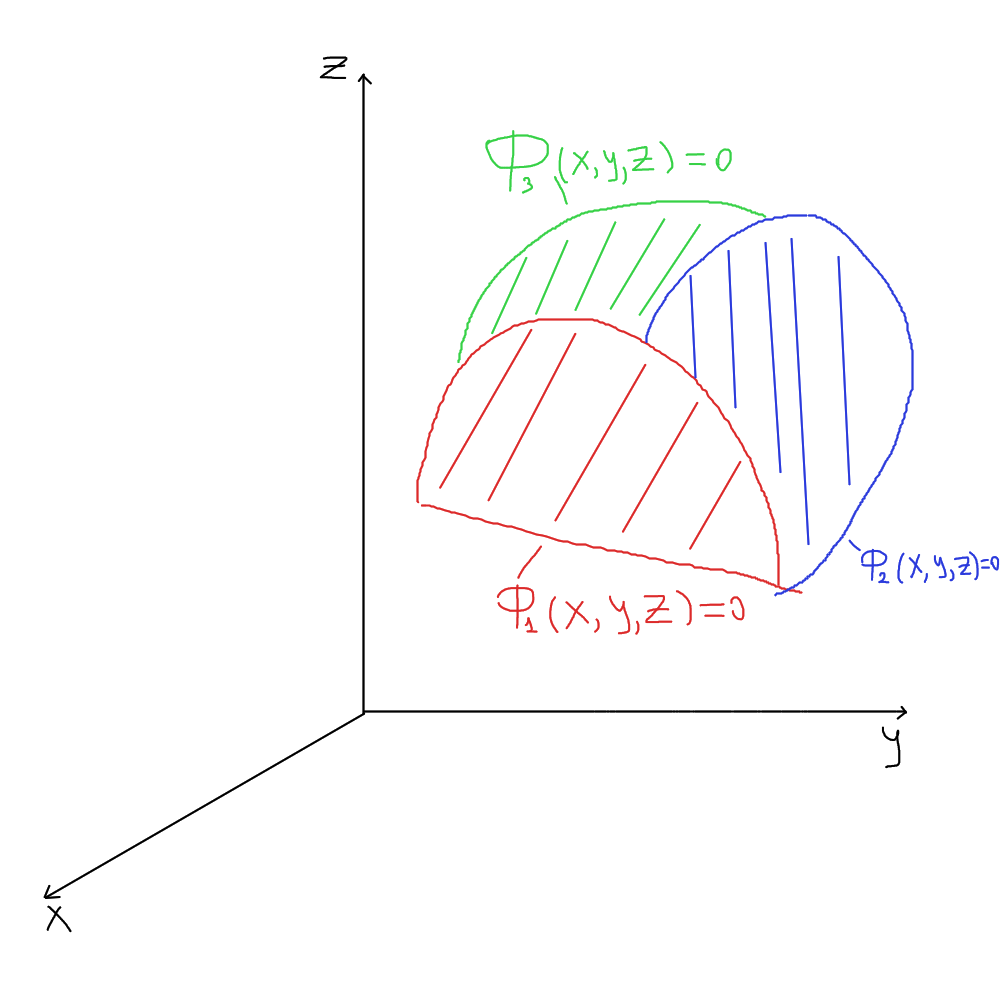
\includegraphics[width=10cm]{pics/1.png}
                \centering
            \end{figure}
            \[\text{ наиб и наим знач. ф. } \ u = f(x, y, z) \text{ на } E\]
            \begin{enumerate}
                \item внутри $E \Ra \begin{cases}
                    f'_x = 0\\
                    f'_y = 0\\
                    f'_z = 0
                \end{cases}$ - реш. системы\\
                 (только принадлежащие $E$. Решения могут лежать вне $E$)\\
                 Или точка недифф.
                \item На участке $\Phi_1(x, y, z) = 0$
                    \begin{enumerate}
                        \item точка недифф-ти
                        \item $\rk \Phi_1' < 1$
                        \item $\LL = f - \lambda_1 \Phi_1$
                    \end{enumerate}
                    <<Не нужно считать 2 пр-дные и делать лишнее!>>
                \item На участке $\Phi_2(x, y, z) = 0$\\
                    Аналогично
                \item На $\Phi_3(x, y, z) = 0$
                    Аналогично
                \item на ребре
                    \[\begin{cases}
                        \Phi_1 = 0\\
                        \Phi_2 = 0
                    \end{cases}\]
                    \begin{enumerate}
                        \item Не дифф
                        \item $\rk \begin{pmatrix}
                            \Phi'_1\\
                            \Phi'_2
                        \end{pmatrix} < 2$
                        \item $\LL = f - \lambda_1 \Phi_1 - \lambda_2 \Phi_2$
                    \end{enumerate}
                \item на ребре
                \item на ребре
                \item в точках
                    \[\begin{cases}
                        \Phi_1(x, y, z) = 0\\
                        \Phi_2(x, y, z) = 0\\
                        \Phi_3(x, y, z) = 0\\
                    \end{cases}\]
            \end{enumerate}
            \hline
            \[\]
            Все точки проверяем на $\in $ E\\
            $f(x_1, y_1, z_1), f(x_2, y_2, z_2), ...$ выбираем точку с
            $\us{\text{наим}}{\text{наиб}}$ знач.
        \end{Definition} 

        \begin{Task}[1]
            \[z = x^2 - xy + y^2\]
            на мн-ве\ $\{(x, y) : \ \abs{x} + \abs{y} \leq 1\}$
            \[1)\]
            \begin{figure}[H]
                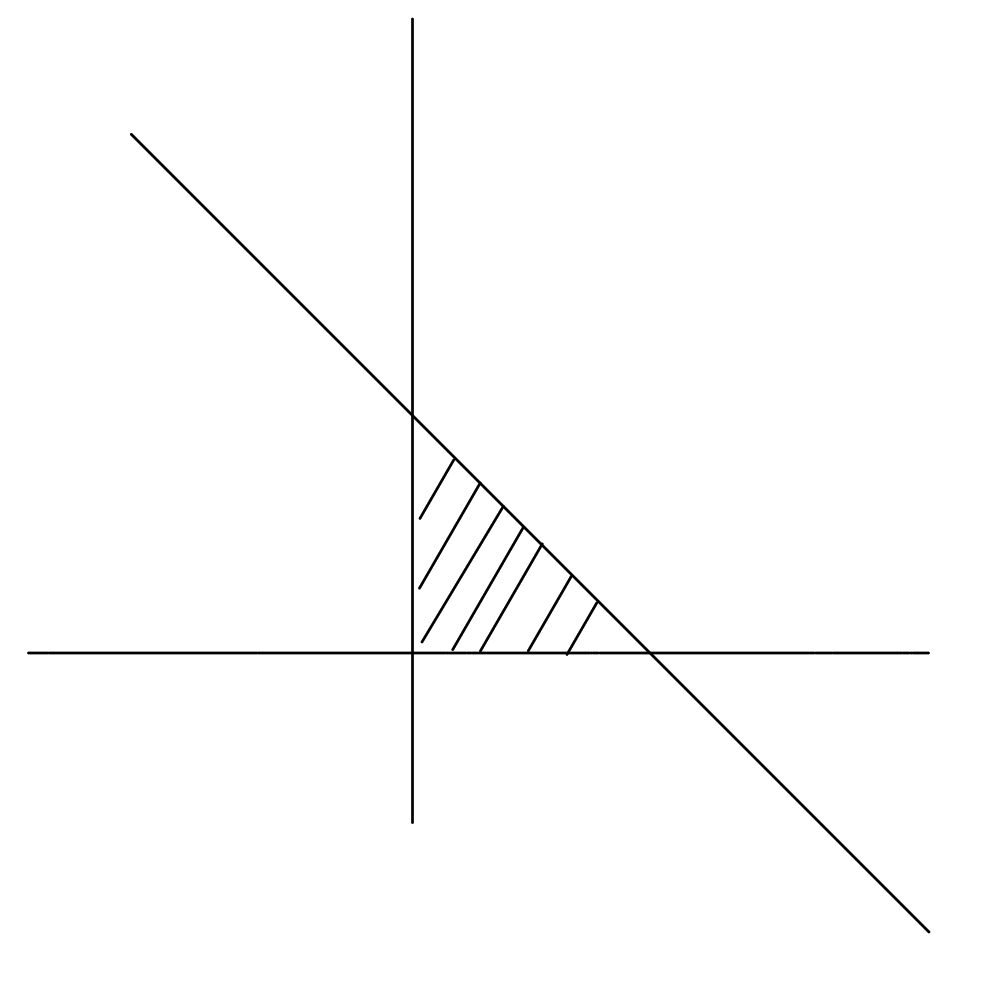
\includegraphics[width=3cm]{pics/2}
                \centering
            \end{figure}
            \[x \geq 0\]
            \[y \geq 0\]
            \[x + y \leq 1\] 
            \[2)\]
            \begin{figure}[H]
                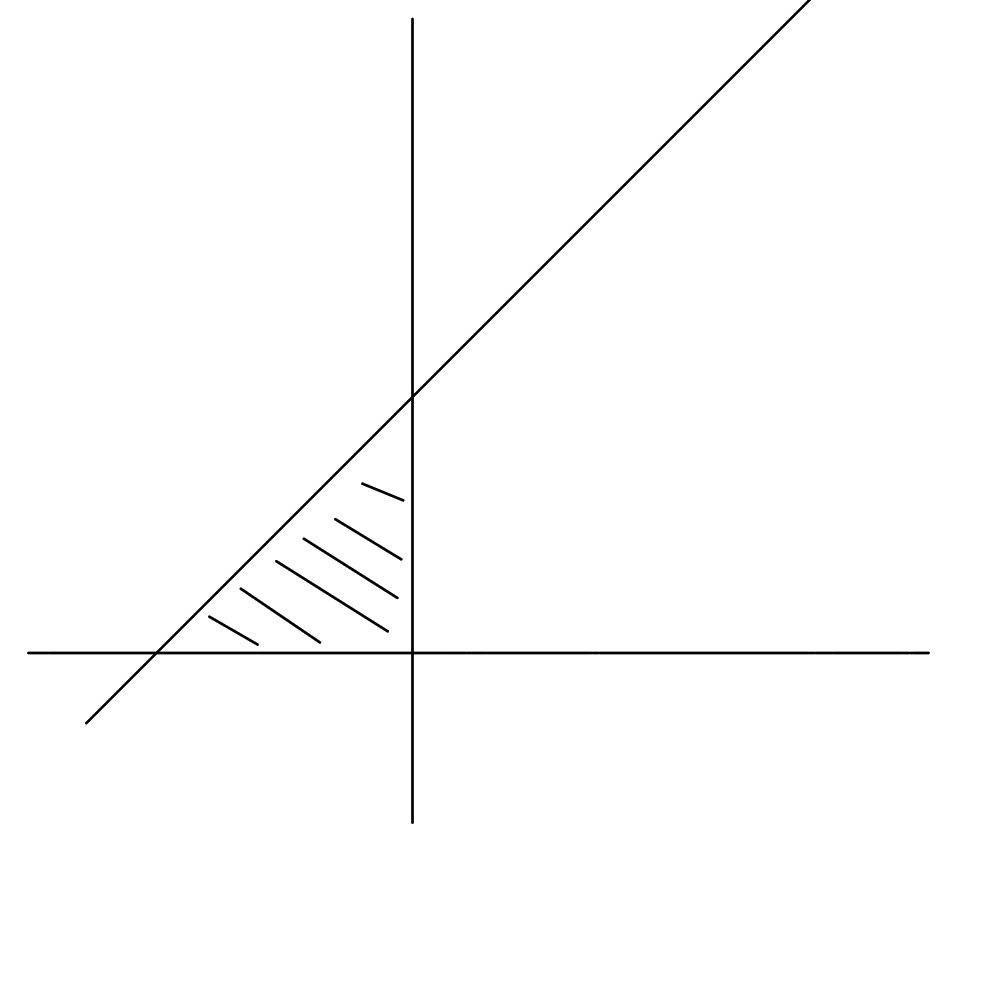
\includegraphics[width=3cm]{pics/3}
                \centering
            \end{figure}
            \[x < 0\]
            \[y \geq 0\]
            \[-x + y \leq 1\]
            \[3)\]
            \begin{figure}[H]
                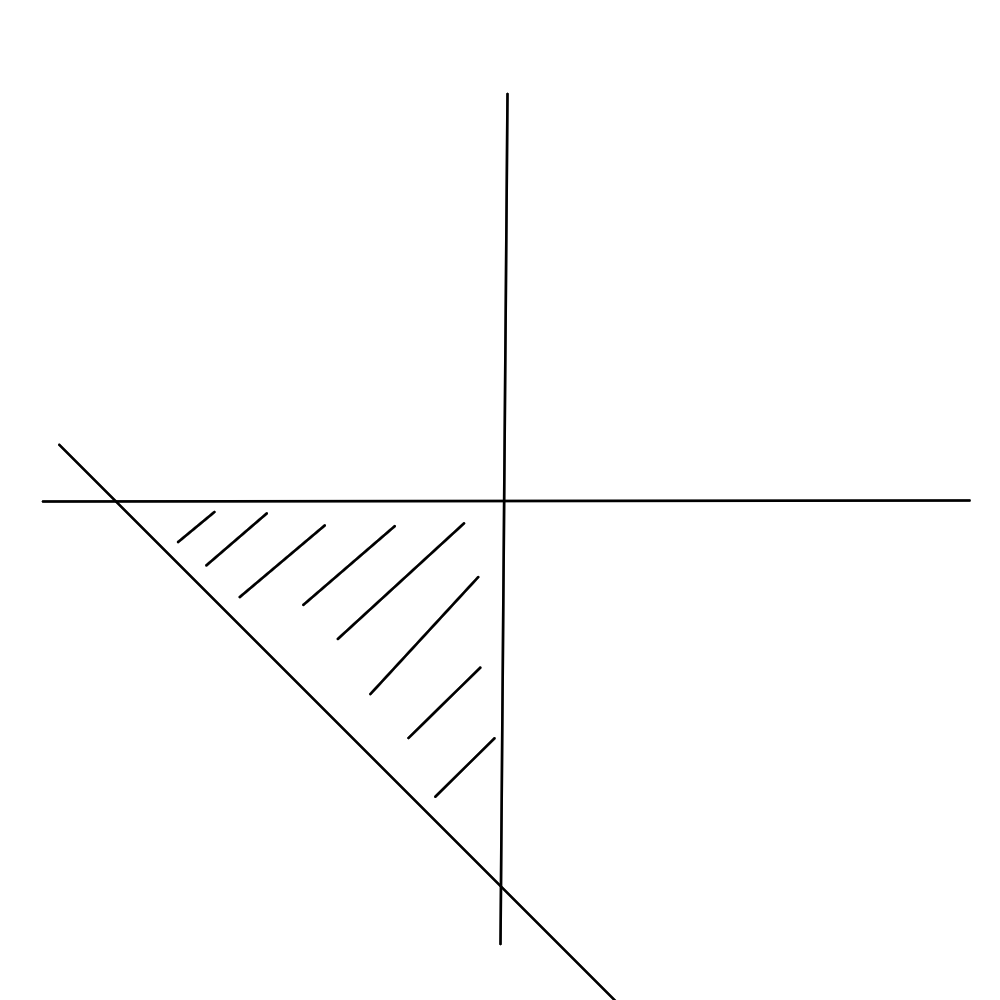
\includegraphics[width=3cm]{pics/4}
                \centering
            \end{figure}
            \[x < 0\]
            \[y < 0\]
            \[-x - y \leq 1\]
            \[4)\]
            \begin{figure}[H]
                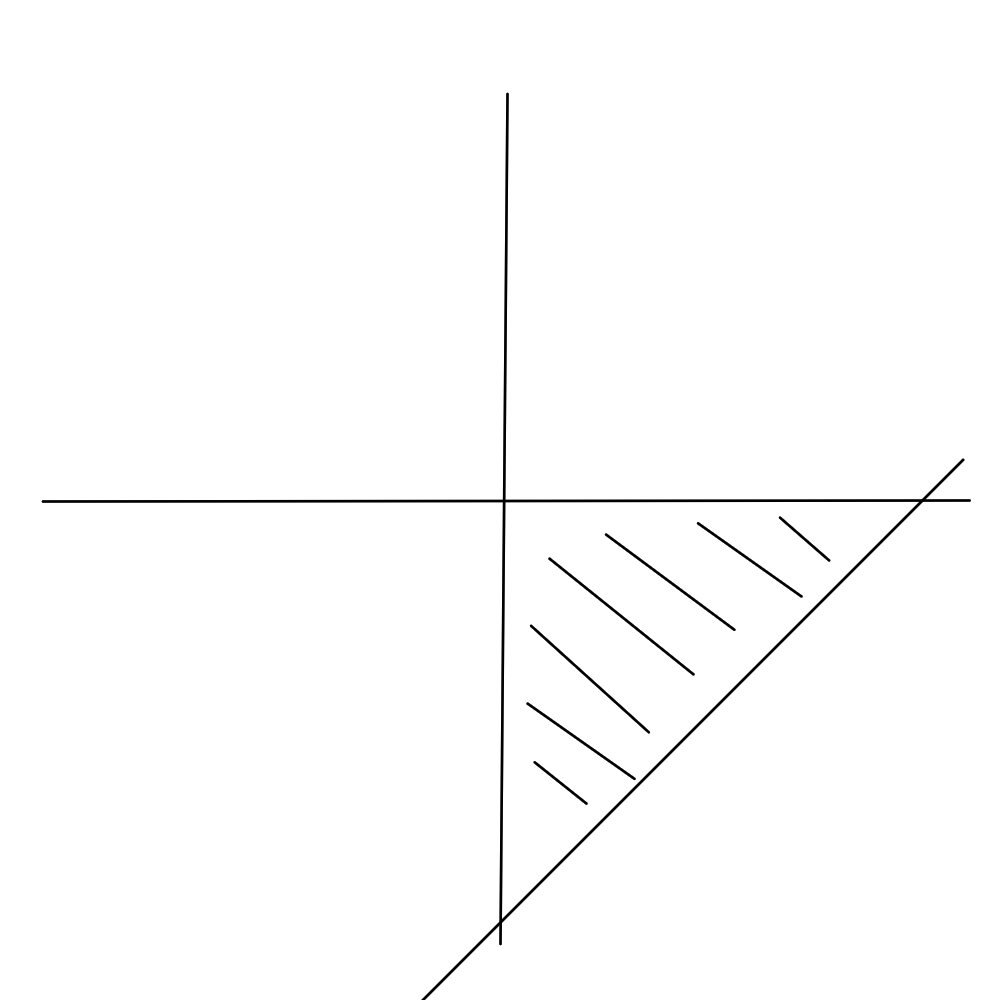
\includegraphics[width=3cm]{pics/5}
                \centering
            \end{figure}
            \[x \geq 0\]
            \[y < 0\]
            \[x - y \leq 1\]
            \begin{figure}[H]
                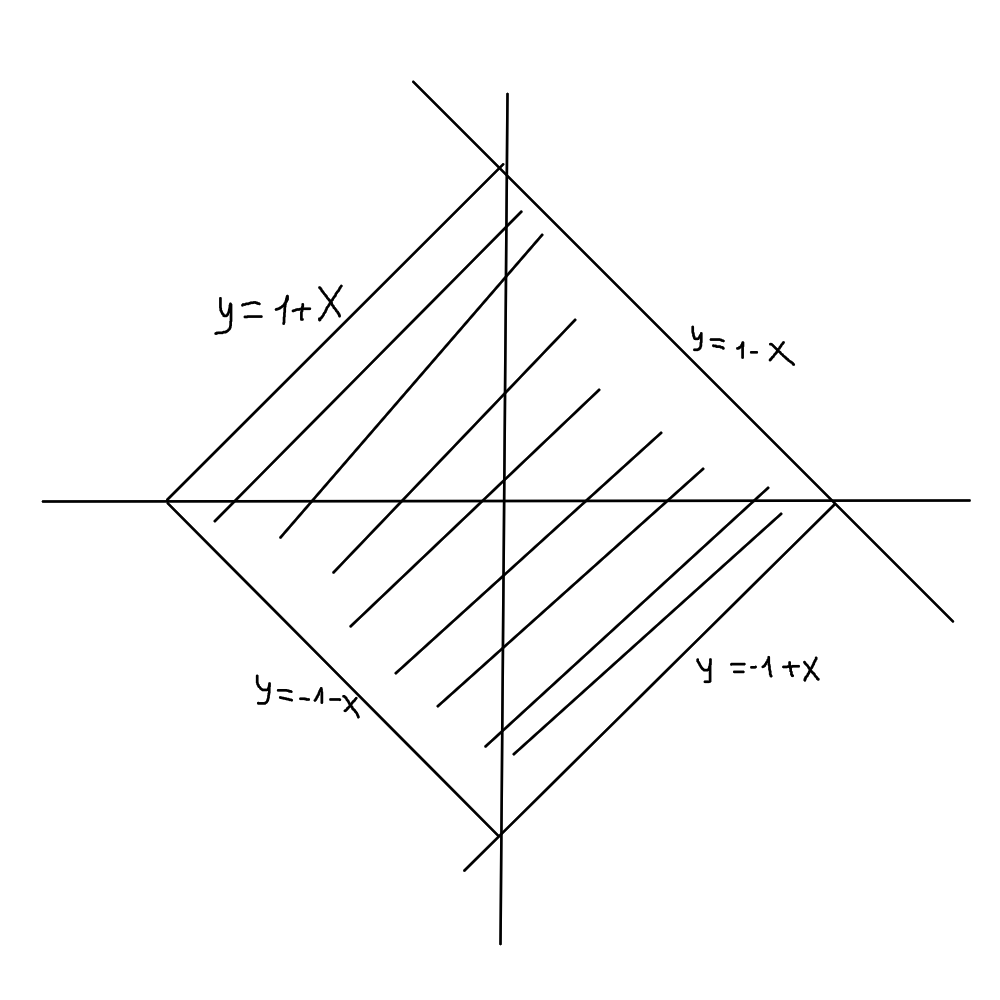
\includegraphics[width=7cm]{pics/6.png}
                \centering
            \end{figure}
            \[1) внутри\]
            \[z'_x = 2x - y = 0\]
            \[z'_y = -x + 2y = 0\]
            \[\begin{cases}
                2x - y = 0 \\
                -x + 2y = 0
            \end{cases} \qq \begin{cases}
                y = 2x\\
                4x - x = 0
            \end{cases} \qq \begin{cases}
                y = 0\\
                x = 0
            \end{cases} \text{ входит в множество}\]
            \hline
            \[2)\]
            \[\begin{cases}
                y = 1 - x\\
                z = x^2 - x(1 - x) + (1 - x)^2
            \end{cases} \rla \begin{cases}
                y = 1 - x\\
                z = 3x^2 - 3x + 1
            \end{cases}\]
            \[z'_x = 6x - 3 = 0\]
            \[\begin{cases}
                y = \frac{1}{2}\\
                x = \frac{1}{2}
            \end{cases} \text{ входит в мн-во}\]
            \hline
            \[3)\]
            \[\begin{cases}
                y = x - 1\\
                z = x^2 - x(x - 1) + (x - 1)^2
            \end{cases}\]
            \[z'_x = 2x - 1 = 0\]
            \[\begin{cases}
                x = \frac{1}{2}\\
                y = -\frac{1}{2}
            \end{cases}\]
            Догадались о симметрии
            \[\begin{cases}
                x = - \frac{1}{2}\\
                y = - \frac{1}{2}
            \end{cases}\]
            \[\begin{cases}
                x = -\frac{1}{2}\\
                y = \frac{1}{2}
            \end{cases}\]
            Входят в множество
            \hline
            \[4) точки пересечения границ\]
            \[\begin{cases}
                x = 1\\
                y = 0
            \end{cases} \q \begin{cases}
                x = -1\\
                y = 0
            \end{cases} \q \begin{cases}
                x = 0\\
                y = 1
            \end{cases} \q \begin{cases}
                x = 0\\
                y = -1
            \end{cases}\]
            \[z(0, 0) = 0 \la \min\]
            \[z\left(\frac{1}{2}, \frac{1}{2}\right) = \frac{1}{4}\]
            \[z\Br{-\frac{1}{2}, -\frac{1}{2}} = \frac{1}{4}\]
            \[z\Br{\frac{1}{2}, -\frac{1}{2}} = \frac{3}{4}\]
            \[z\Br{-\frac{1}{2}, \frac{1}{2}} = \frac{3}{4}\]
            \[z(1, 0) = 1\]
            \[z(-1, 0) = 1\]
            \[z(0, 1) = 1\]
            \[z(0, -1) = 1 \la \max\]
        \end{Task}

        \begin{Task}[2 Найти $\max \q \min$]
            \[u = x + y + 2z\]
            на мн-ве $\{(x, y, z) \ | \ x^2 + y^2 \leq (z - 1)^2, \q (z \leq 1),
            \q z \geq x ^ 2 + y\}$
            \[x^2 + y^2 \leq (z - 1)^2 \text{ - конус}\]
            \begin{figure}[H]
                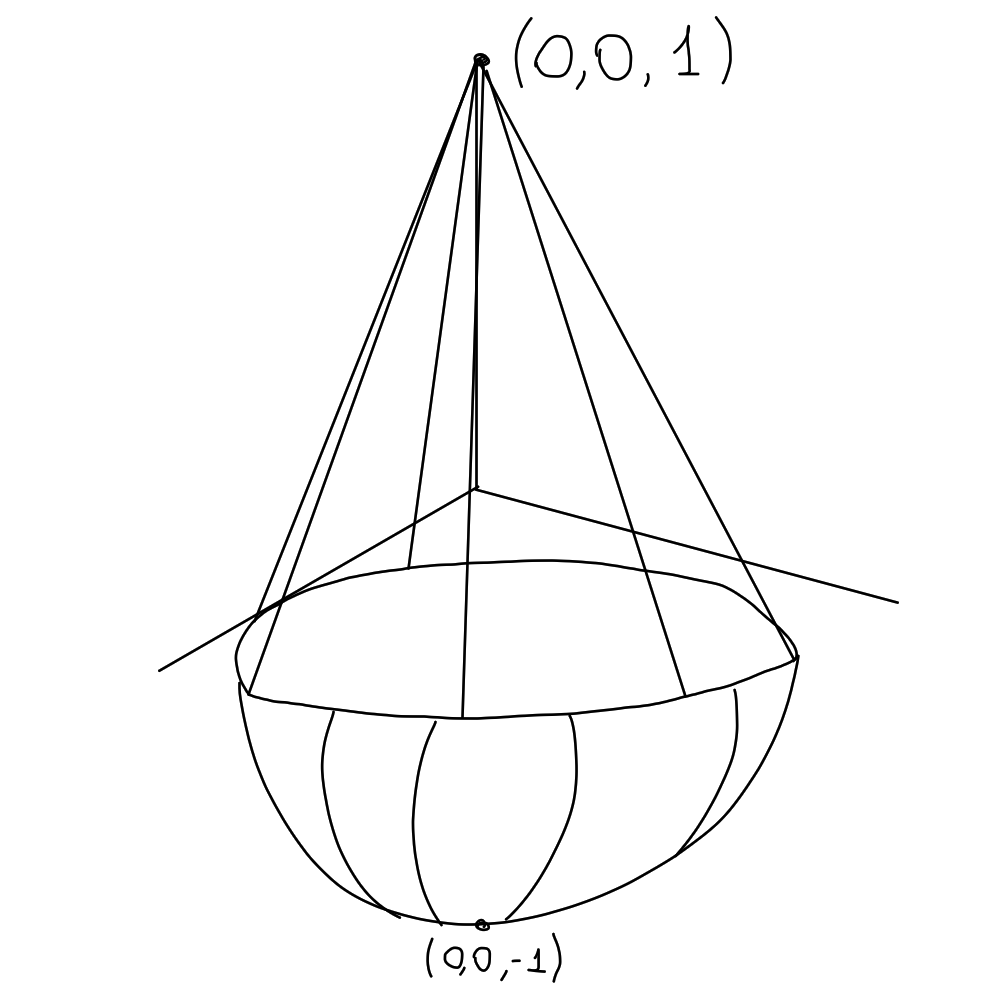
\includegraphics[width=7cm]{pics/7.png}
                \centering
            \end{figure}
            \[1)\]
            \[\begin{cases}
                u'_x = 1 & \neq 0\\
                u'_y = 1 & \neq 0\\
                u'_z = 2 & \neq 0
            \end{cases}\]
            Внутри точек нет
            \[2) \q \text{ на } x^2 + y^2 - (z - 1)^2 = 0\]
            \[\rk \begin{pmatrix}
                2x & 2y & -2(z - 1)
            \end{pmatrix} < 1\]
            \[x = 0 \q y = 0 \q z = 1 \text{  на пов-ти}\]
            \[\begin{cases}
                x = 0\\
                y = 0\\
                z = 1
            \end{cases} \in E\]
            
            \[\begin{cases}
                 \LL = x + y + 2z - \lambda(x^2 + y^2 - (z - 1)^2) \\
                 \LL_x' = 1 - 2x\lambda = 0\\
                 \LL_y' = 1 - 2y\lambda = 0\\
                 \LL_z' = 2 + 2\lambda(z - 1) = 0
            \end{cases}\]
            \[x = \frac{1}{2\lambda}\]
            \[y = \frac{1}{2\lambda}\]
            \[y - 1 = - \frac{1}{\lambda}\]
            \[\frac{1}{4\lambda^2} + \frac{1}{4\lambda^2} = \frac{1}{\lambda^2}\]
            \[1 + 1 = 4 \q \cancel{\exists }\]
            
            \[3) \text{  на } x^2 + y^2 - z - 1 = 0\]
            \[\Phi' = \begin{pmatrix}
                2x,& 2y, & -1 
            \end{pmatrix}\]
            \[\rk \Phi' = 1\]
            \[\LL = x + y + 2z - \lambda(x^2 + y^2 - z - 1)\]
            \[\begin{cases}
                \LL'_x = 1 - 2\lambda x = 0 & x = \frac{1}{2\lambda} = -\frac{1}{4}\\
                \LL'_y = 1 - 2\lambda y = 0 & y = \frac{1}{2\lambda} = -\frac{1}{4}\\
                \LL'_z = 2 + \lambda = 0 & \lambda = - 2\\
                x^2 + y^2 - z - 1 = 0
            \end{cases}\]
            \[\frac{1}{16} + \frac{1}{16} - 1 = z \qq z = - \frac{14}{16} = - \frac{7}{8}\]
            \[\begin{cases}
                x = -\frac{1}{4}\\
                y = -\frac{1}{4}\\
                z = -\frac{7}{8}
            \end{cases}\]
            \[4)\]
            \[\begin{cases}
                x^2 + y^2 - (z - 1)^2 = 0\\
                x^2 + y^2 - z  - 1 = 0
            \end{cases}\]
            \[\begin{pmatrix}
                2x & 2y & -2(z - 1)\\
                2x & 2y & -1
            \end{pmatrix}\]
            \[\Delta_1 = \begin{vmatrix}
                2x & 2y\\
                2x & 2y
            \end{vmatrix} = 0\]
            \[\Delta_2 = \begin{vmatrix}
                2x & -2(z - 1)\\
                2x & -1
            \end{vmatrix} = -2x + 4x(z - 1) =  2x( -1 + 2z - 2) = 2x(2z - 3) = 0\]
            \[\Delta_3 = \begin{vmatrix}
                2y & -2(z - 1)\\
                2y & -1
            \end{vmatrix} = 2y(2z - 3) = 0\]
            \[1) \begin{matrix}
                x = 0\\
                y = 0\\
                z = -1
            \end{matrix}\]
            \[1 \text{ - ур не вып.}\]
            \[2) \begin{matrix}
                z = \frac{3}{2}
            \end{matrix}\]
            Но $z \leq 1$ не входит в $E$
            \[5)\]
             \[\LL = x + y + 2z - \lambda_1(x^2 + y^2 - (z - 1)^2) - \lambda_2(x^2 + y^2 - z - 1)\]
             Закончить дома
        \end{Task}
        Дз 3657 б\\
        3663 а\\
        3668
    \end{lect} 
\end{document}

